\documentclass[a4paper,12pt]{article}

% --- Präambel ---
\usepackage[ngerman]{babel}
\usepackage{fontspec}
\usepackage{amsmath}
\usepackage{graphicx}
\usepackage{booktabs}
\usepackage{csquotes}
\usepackage[backend=biber,style=authoryear]{biblatex}
\addbibresource{literatur.bib}

\title{Mini-Dokumentation: Geschwindigkeitsmessung}
\author{Dein Name}
\date{\today}

\begin{document}
\maketitle
\tableofcontents

\section{Einleitung}
Diese Mini-Dokumentation zeigt die wichtigsten Bausteine von \LaTeX{}:
Gliederung, Aufzählung, Abbildung, Tabelle, Formel und Literaturverweis.
Die Erfolgsquote der Testläufe beträgt 95\%; die Rohdaten liegen in
der Datei \texttt{messung\_01.txt}. % Sonderzeichen maskiert

Der Satz selbst wurde mit \LaTeX{} gesetzt (\parencite{knuth1984}); die
verwendeten Pakete sind bei CTAN dokumentiert \parencite{ctan2026biblatex}.

\section{Aufbau}

\subsection{Entwicklungsumgebung}
Für die Dokumentation werden folgende Werkzeuge verwendet:
\begin{itemize}
  \item \emph{VS Code} mit der Erweiterung LaTeX Workshop
  \item \emph{MiKTeX} als \LaTeX-Distribution
  \item \emph{Biber} zur Verarbeitung der Literaturdaten
\end{itemize}

\subsection{Systemaufbau}
Der prinzipielle Aufbau ist in Abbildung~\ref{fig:system} dargestellt.
Die Messwerte stehen in Tabelle~\ref{tab:messung}.

\begin{figure}[htbp]
  \centering
  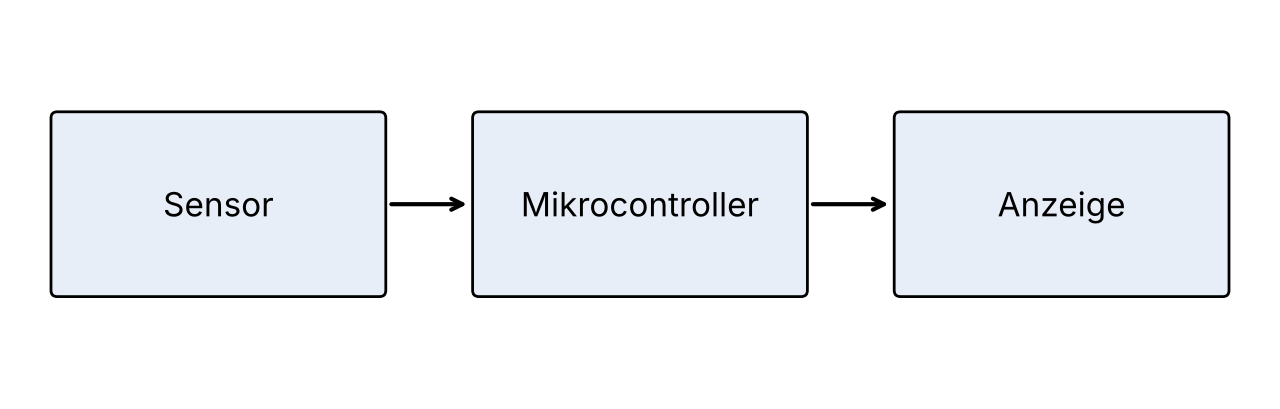
\includegraphics[width=.8\textwidth]{bilder/system.png}
  \caption{Aufbau des Messsystems}
  \label{fig:system}
\end{figure}

\begin{table}[htbp]
  \centering
  \caption{Messwerte der Geschwindigkeit}
  \label{tab:messung}
  \begin{tabular}{lcc}
    \toprule
    Messung & Soll (m/s) & Ist (m/s) \\
    \midrule
    1 & 2,0 & 1,9 \\
    2 & 4,0 & 4,1 \\
    3 & 6,0 & 5,8 \\
    \bottomrule
  \end{tabular}
\end{table}

\section{Auswertung}
Die Geschwindigkeit ergibt sich nach Gleichung~\ref{eq:geschwindigkeit}
aus Weg und Zeit:
\begin{equation}
  v = \frac{s}{t}
  \label{eq:geschwindigkeit}
\end{equation}
Zusätzlich gilt für die Fläche eines Kreises (Gleichung~\ref{eq:kreis}):
\begin{equation}
  A = \pi r^{2}
  \label{eq:kreis}
\end{equation}

\printbibliography
\end{document}
